\documentclass[11pt]{article}

\title{Dimensionality reduction \\ - \\ Concepts and applications in scRNA-seq and DNA microscopy}
\author{Gergo Bohner}

\usepackage{graphicx}
\graphicspath{{fig/}}

\begin{document}

\maketitle


Dimensionality reduction is a widely applied set of methods in various data analysis pipelines. It has three main aims:

\begin{itemize}
	\item \emph{Describe the data manifold} \\ Parametrise a space that we believe the observed data lives in. This space also serves as generalisation of where we expect future data to show up. Furthermore certain parameterisations - together with information not contained in the dataset - may facilitate interpretation of features.
	\item \emph{Reduce the observation noise} \\ We may separate the data variance into "within-manifold" (signal) and "out-of-manifold" (noise).
	\item \emph{Visualise the concepts discovered in the data} \\ Most collected data nowadays is very high (100+) dimensional, whereas most humans can only conceptualise a few dimensions at once. We have the responsibility to choose the most effective, yet accurate visualisations of the data to communicate features of the data
\end{itemize} 

These goals are often interspersed, yet both the researcher and their audience should be clear on why a dimensionality reduction method was applied, even when the mathematical methodology to achieve each goal may be the exact same.


\begin{itemize}
	\item \emph{Manifold learning} (e.g. Isomap) \\ Estimate within-manifold distances, predict what data is likely in the future, learn about structure embedded within the data
\end{itemize}

\begin{figure}[h!]
\centering
\hspace{-4cm}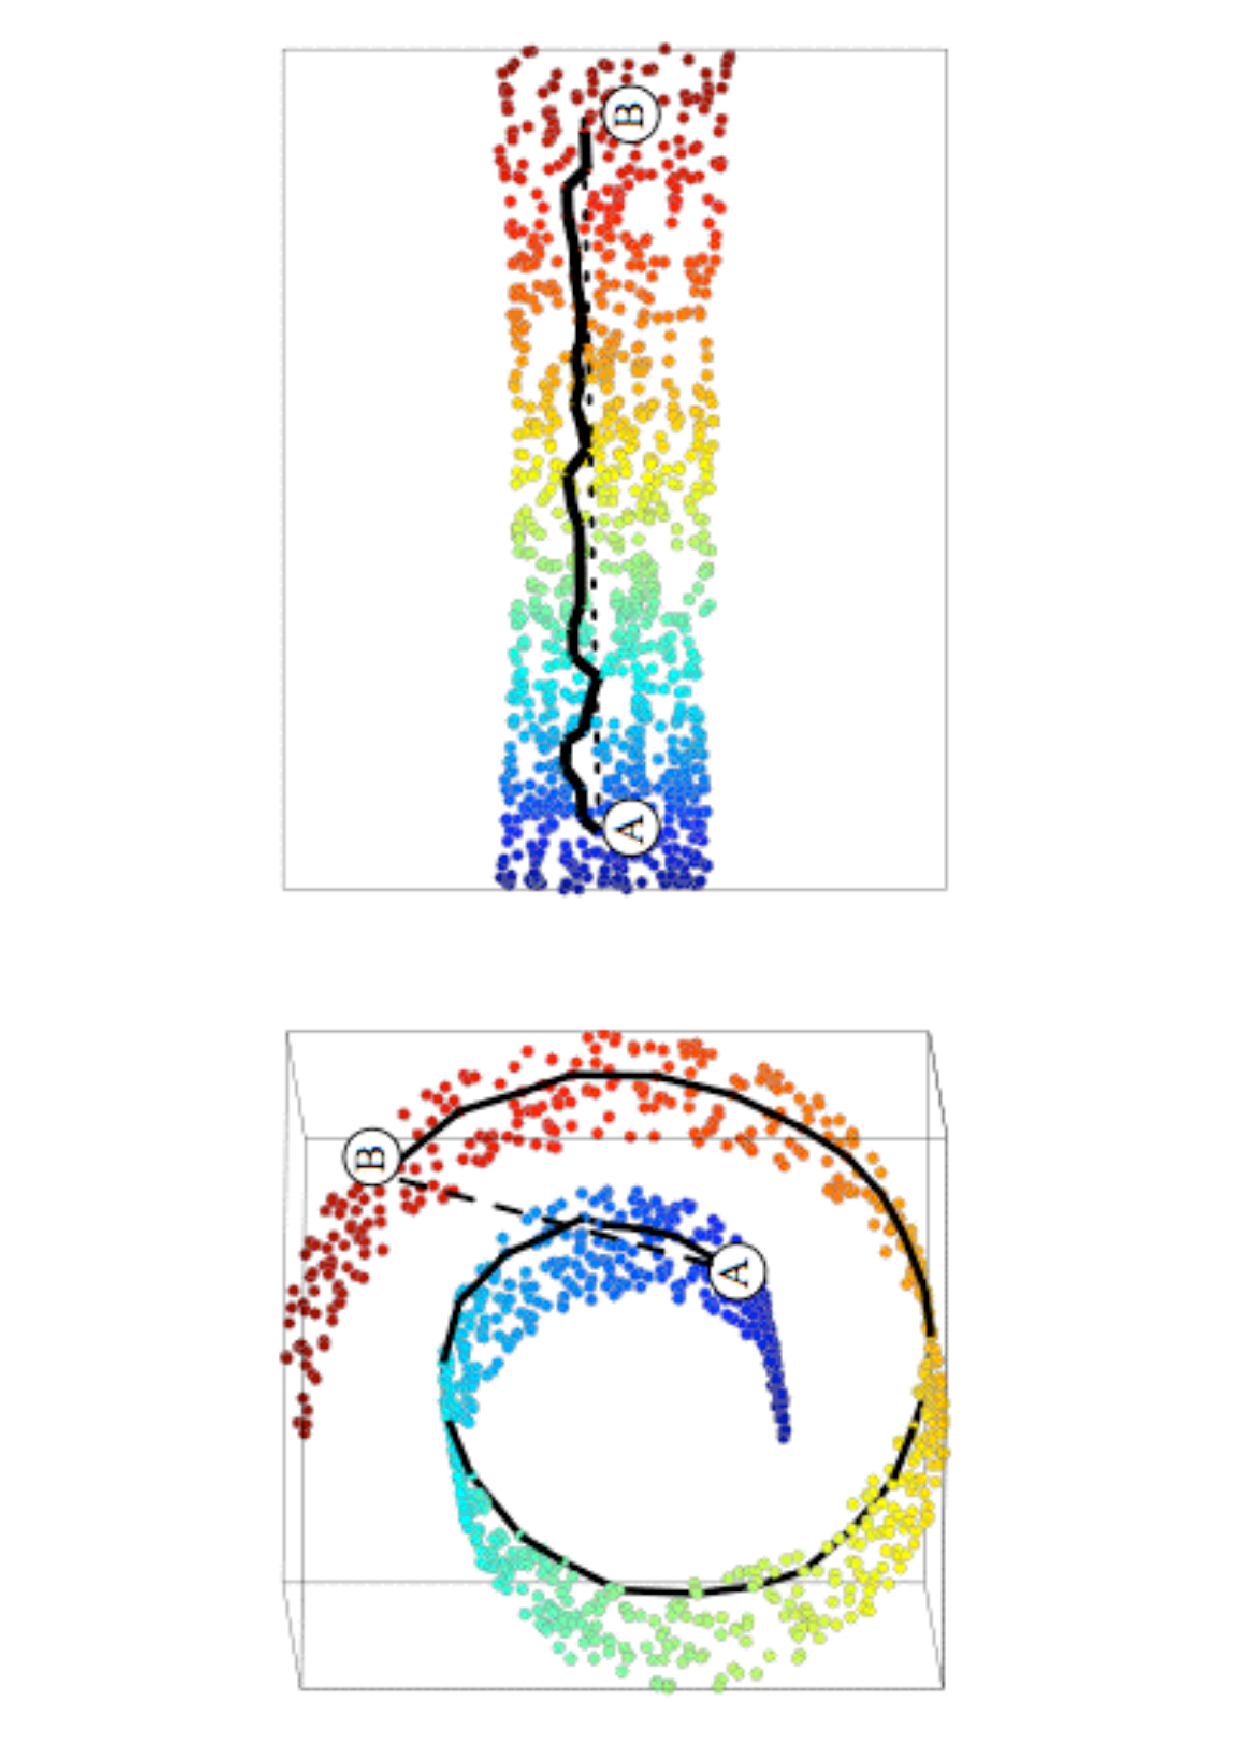
\includegraphics[angle=-90,origin=c, height=0.7\linewidth, width=0.23\textwidth]{swiss-unroll-distance}
\\ \vspace{-7cm}
\includegraphics[width=0.5\linewidth]{bat_neurons_nature14031-f3} 
\caption{Examples for manifold estimation. (top) Swiss roll artificial dataset shows the concepts of a 2D manifold embedded in 3D (color purely serves as visual aid). (bottom) Comparing different manifold hypotheses (spherical vs toroidal) in behaving bats to explain neural variability \emph{(Finkelstein et al, Nature 2015)}}
\end{figure} 


\begin{itemize}
	\item \emph{Feature discovery} (e.g. PCA, ICA) \\ Find a meaningful "basis" for the manifold - a set of features whose combination explains the data well, and 
\end{itemize}

\begin{itemize}
	\item \emph{Reduce observation noise} (e.g. PCA, pPCA, FA) \\ TODO
\end{itemize}

\begin{itemize}
	\item \emph{Visualise high-D data} (e.g. t-SNE) \\ TODO
\end{itemize}


\section{Linear methods}

  %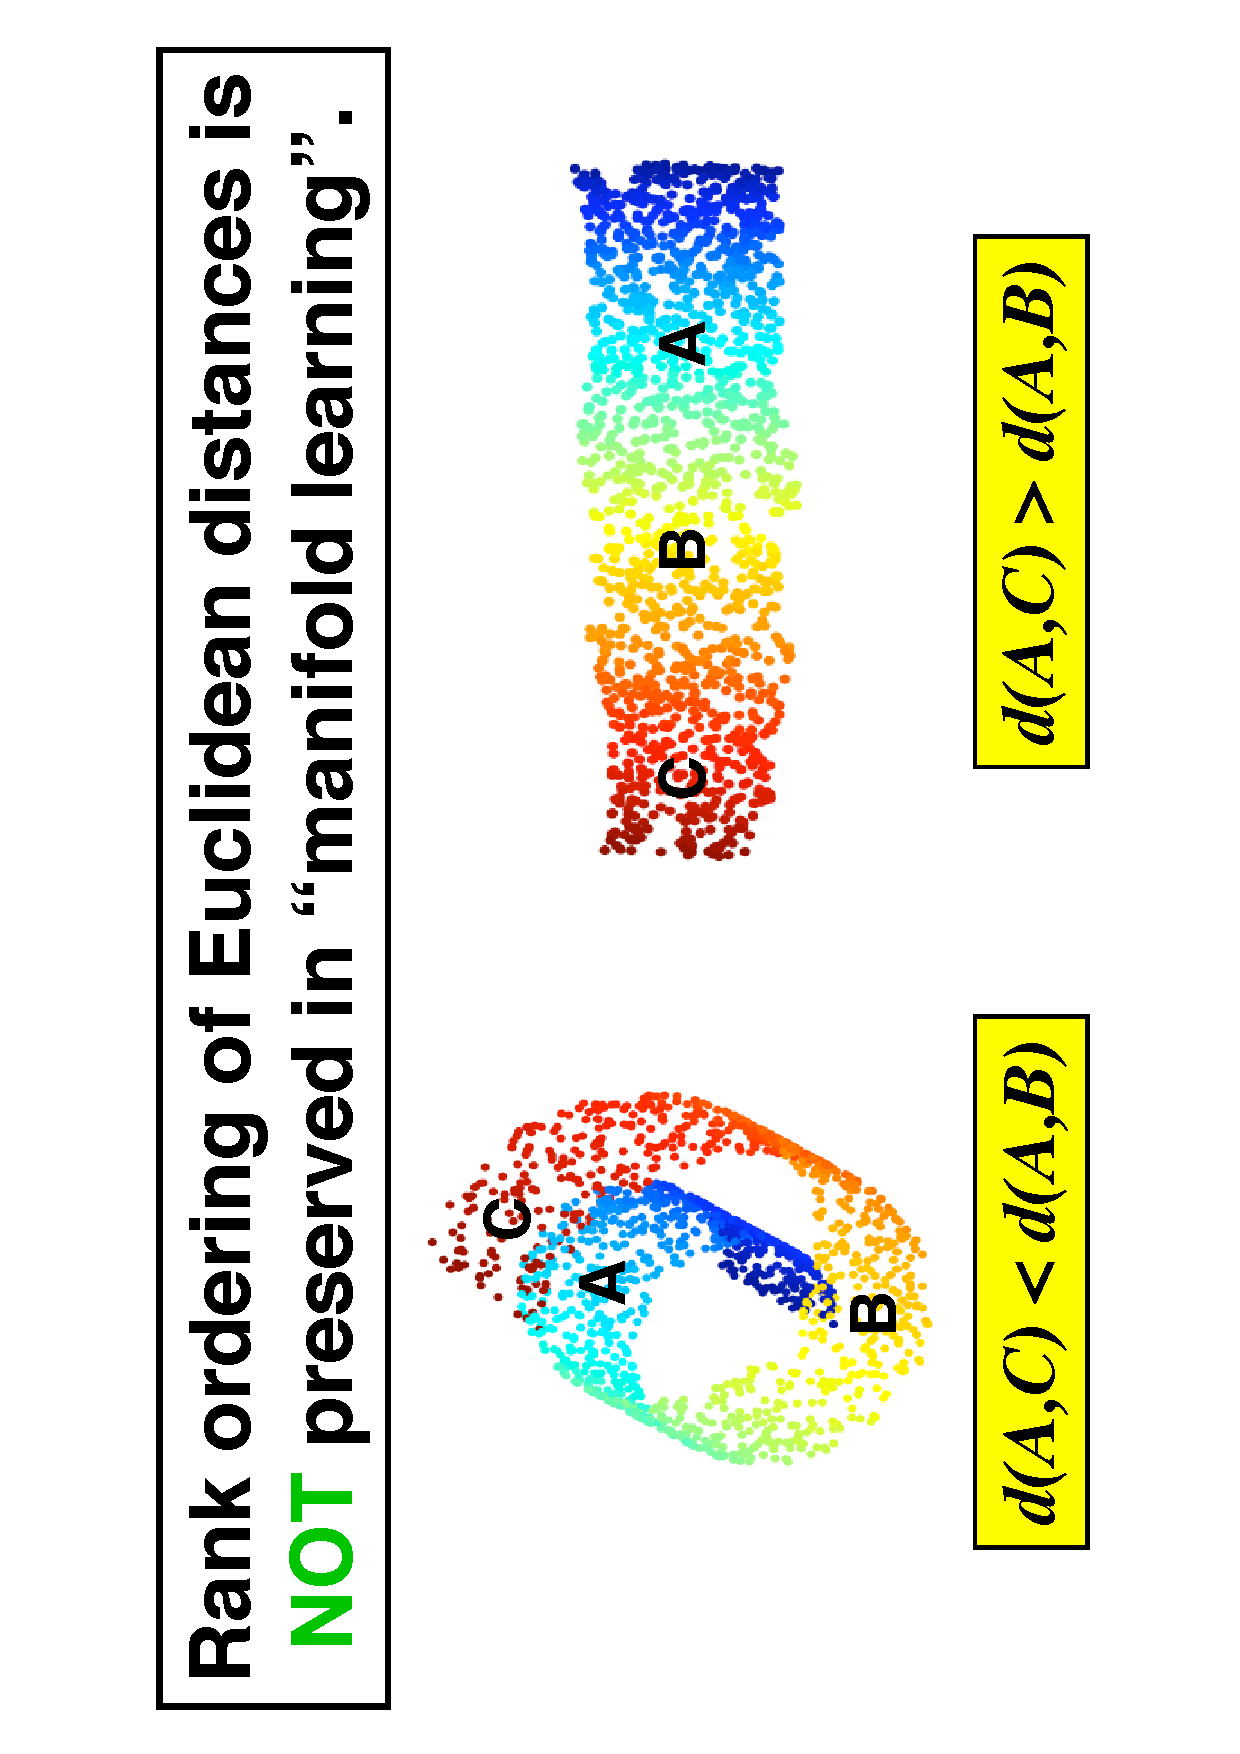
\includegraphics[angle=-90,origin=c, height=0.6\textwidth, width=0.2\textwidth]{rank-order-not-preserved.pdf}



\end{document}
